\section{问题定义与研究内容}

\subsection{研究对象}

变截面杆的轴向响应可以用一维理论以极低代价估算，但其端部与截面内的二维效应会随锥角增大而迅速增强。本文研究一个截面高度沿杆轴线性变化、关于杆轴对称的矩形拉杆：杆轴取 $x$ 轴，$x\in[0,L]$；矩形截面的面外宽度（厚度）$b$ 恒定，面内高度为
\begin{equation}
  h(x)=h_0\left(1+\beta\frac{x}{L}\right),\qquad
  \beta=\frac{h_1-h_0}{h_0},
  \label{eq:taper}
\end{equation}
截面范围为 $y\in[-h(x)/2,\,h(x)/2]$。采用关于杆轴对称、而非“平底楔形”的几何，是为了让截面形心线保持为直线 $y=0$，端部均布轴力的合力通过形心线，不引入额外整体弯曲；$\beta=0$ 即退化为等截面矩形杆。几何与材料参数见表~\ref{tab:params}。

\begin{table}[htbp]
  \centering
  \caption{几何与材料参数。所有量取国际单位制。}
  \label{tab:params}
  \small
  \setlength{\tabcolsep}{3pt}
  \begin{tabular}{@{}llll@{}}
\toprule
参数 & 符号 & {取值} & 单位 \\
\midrule
杆长 & $L$ & 1.0 & m \\
固定端高度 & $h_0$ & 0.2 & m \\
面外厚度 & $b$ & 0.1 & m \\
弹性模量 & $E$ & $2.0\times10^{11}$ & Pa \\
泊松比 & $\nu$ & 0.3 & -- \\
端部总拉力 & $P$ & 1000 & N \\
平面应力厚度 & $t=b$ & 0.1 & m \\
\bottomrule
\end{tabular}

\end{table}

\begin{figure}[htbp]
  \centering
  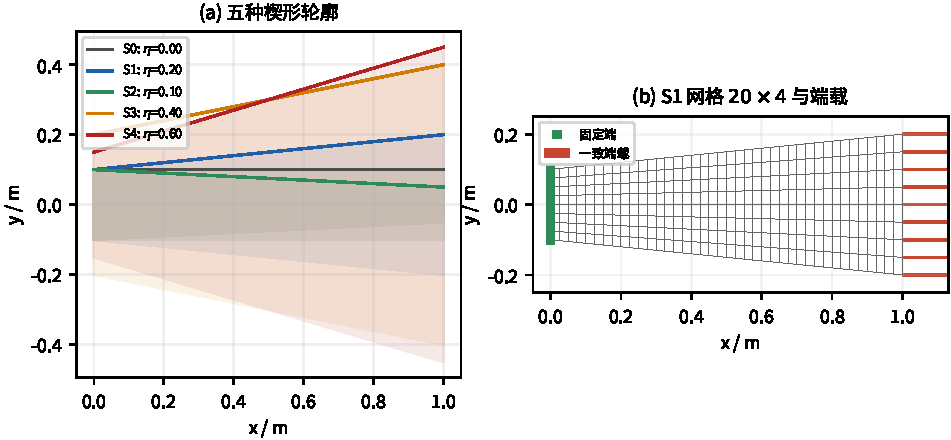
\includegraphics[width=\textwidth]{figures/fig01_geometry_mesh.pdf}
  \caption{五种工况的对称楔形轮廓与 S1 的计算网格。现象：轮廓关于 $y=0$ 对称，网格随 $h(x)$ 缩放，斜边保持直线。解读：对称几何使端部载荷合力通过形心线，避免附加弯曲；沿锥度缩放的网格使单元保持近似正交，便于把锥度效应与网格畸变效应分开。}
  \label{fig:geometry}
\end{figure}

\subsection{计算工况}

主构型 S1 取 $\beta=+1.0$，高度由 $0.2\,\mathrm{m}$ 增至 $0.4\,\mathrm{m}$；S0 为 $\beta=0$ 的退化校核；S2 为收缩楔形，S3、S4 为粗短/极端楔形，用于把一维判据推到 A/B/C 边界。五种工况见表~\ref{tab:cases}。

\begin{table}[htbp]
  \centering
  \caption{五种计算工况。$\eta=|\beta|h_0/L$ 为锥角正切，$A_1/A_0$ 为端部与固定端面积比。}
  \label{tab:cases}
  \small
  \begin{tabular}{@{}lS[table-format=+1.2]S[table-format=1.2]S[table-format=1.2]S[table-format=1.2]S[table-format=2.1]S[table-format=1.2]@{}}
\toprule
工况 & {$\beta$} & {$h_0$/m} & {$h_1$/m} & {$\eta=|\beta|h_0/L$} & {锥角/$^\circ$} & {$A_1/A_0$} \\
\midrule
S0 & +0.00 & 0.20 & 0.20 & 0.00 & 0.0 & 1.00 \\
S1 & +1.00 & 0.20 & 0.40 & 0.20 & 11.3 & 2.00 \\
S2 & -0.50 & 0.20 & 0.10 & 0.10 & 5.7 & 0.50 \\
S3 & +1.00 & 0.40 & 0.80 & 0.40 & 21.8 & 2.00 \\
S4 & +2.00 & 0.30 & 0.90 & 0.60 & 31.0 & 3.00 \\
\bottomrule
\end{tabular}

\end{table}

\subsection{边界条件与载荷}

固定端 $x=0$ 全部节点满足 $u_x=u_y=0$；加载端 $x=L$ 施加沿 $x$ 方向的均布轴向拉力，合力 $P=1000\,\mathrm{N}$；上下斜边自由。二维模型采用平面应力，厚度 $t=b=0.1\,\mathrm{m}$。

端部载荷采用\textbf{均布轴向拉力的一致节点载荷}，而非“每个端节点等分 $P$”的集中载荷：线性边每个微段的面力合力一半分给两端节点，角点因此为内点的一半；CPS8 则按 $1/6$–$2/3$–$1/6$ 分配。两种口径对 $u_{\rm end}$ 的影响不超过 $0.28\%$，但对加载端局部节点应力可达 $1\%$–$8\%$，因此点值应力对比时必须统一。本文所有结果均采用一致面力口径，敏感性在 \S\ref{sec:anchor} 中量化。

\subsection{研究内容}

等参元与常应变三角形的标准推导可参考经典教材~\cite{zienkiewicz2005,bathe2006,hughes2000}。本文完成四项工作。第一，自写 Python+NumPy/SciPy 有限元程序，实现一维变截面杆、Q4 与 CST 的单元刚度、稀疏组装与求解。第二，比较端部/中截面位移、名义应力沿轴曲线与应力误差随网格的 $e$--$\sigma$ 收敛。第三，量化 Q4 的梯度保真误差与剪切能比，以及 CST 的面积加权节点应力恢复与对角线离散度。第四，用 CalculiX CPS4/CPS8 建立第三方锚点，并用 FEniCS 做可选本构校核。三种方法的\textbf{产出形态}差异单列于第~\ref{sec:forms} 节，因为“能输出什么”与“算得多准”同样决定工程选型。